%!TEX root = ./main.tex
\section{Meta-Path Embedding based Recommendation}

\begin{figure*}[!t]
    \centering
    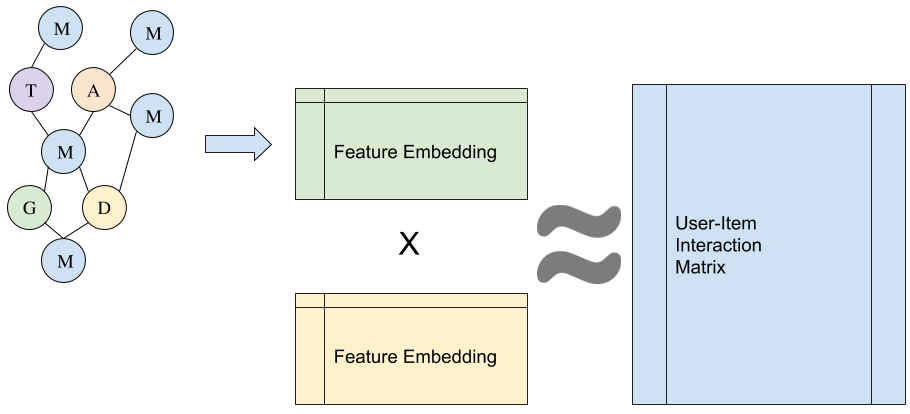
\includegraphics[width=0.8\textwidth]{figs/fig0.png}
    \caption{workflow of MERec}\label{fig:fe-overview}
\end{figure*}

In this Section, we propose MERec that meta-path based embedding and Bayesian Probability Ranking to overcome cold start problem. 

The key idea of our approach is inspired by recent research on graph-based embedding \cite{dong2017metapath2vec}. Unlike traditional matrix based approach, which learns user/item latent representation jointly based on user-item interactions matrix. Our one breaks down item and user latent matrix learning through 2 separate steps. as illustrated in Fig. \ref{fig:fe-overview}. Item embedding is first learned based on item and its features nodes within HIN with a user defined meta-path sets for the moderating its random walk process. Then user latent feature is trained though Factorization Machine, which is optimized by using Bayesian Probability Ranking.

\subsection{Step 1: Item Embedding via Meta-path Based Random Walk}\label{3MF}

For items such as movies, books, music, there are a number of factors impacting users' decision. Instead of taking the one-hot encoding approach for category value. We first propose to treat different categorical information as separate node types. 
By leveraging domain knowledge we can form a heterogeneous information graph and sets of user defined meta-path for item-item similarities learning. 

For example, movie choice is closely linked to directors and its casts. Thus $Movie \rightarrow Director \leftarrow Movie$, $Movie \rightarrow Actor/Actress \leftarrow Movie$  can be very important meta-path in deciding how similar 2 movies are. We use those insights as a guideline to define meta-path from a heterogeneous information graph for item features embedding. As shown in Fig. \ref{fig:fe-graph}.
Each meta-path can derive a item-item similarity matrix $\mathbb{R}_i(\mathcal{P}_i)$, each different meta-path can be regarded as bias toward different feature aspects, so items co-occurrence can be learned separately under different meta-path.

\begin{figure*}[!t]
    \centering
    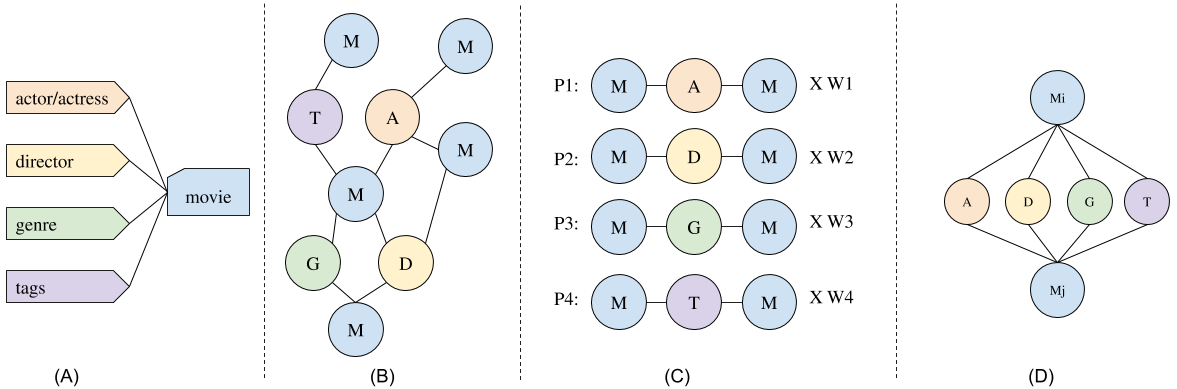
\includegraphics[width=0.8\textwidth]{figs/fig1.png}
    \caption{heterogeneous information graph based on item features}\label{fig:fe-graph}
\end{figure*}

as a result, item-item similarity score can be calculated by normalized meta-path similarity times meta-path weight.
\begin{equation}\label{itemsim}
    \mathcal{S}(v_i,v_j) = 
    \begin{cases}
         \sum\limits_{\substack{n=1}}^{n} \mathcal{R}_ij(\mathcal{P}_n,{W_n}),& \text{if } (v_{i}, .., v_{j}) \in \mathcal{P} \\
         0,              & \text{otherwise}
     \end{cases}
\end{equation}

$\mathcal{S}(v_i,v_j)$ stands for similarity between items $v_i$ and $v_j$ which shares the same node type. $R_ij()$ is a similarity function, where $\mathcal{P}_n, {W_n}$ stands for individual meta-path and its weights respectively. This end result provides guidance for the random walkers on our heterogeneous graph of item features. $(v_{i}, .., v_{j})$ is denoted as a meta-path instance, where $v_i$ is the starting node and $v_j$ the end node.

Given a heterogeneous graph $G = (V,E)$, and a meta-path set $[\mathcal{P}_1, \mathcal{P}_2, ... \mathcal{P}_n]$, the probability of transition is defined as following:
\begin{equation}\label{hetewalker}
    P(v_{i+1},\mathcal{P},w)= 
        \begin{cases}
            p({N^{t+1}(v_{i}^t)}),& \text{if } (v_{i+1}, .., v_{i}^t) \in \mathcal{P} \\
            0,              & \text{otherwise}
        \end{cases}
\end{equation}
where $t$ is denoted as $t^th$ steps, as the walker traversing through the graph and $p({N^{t+1}(v_{i}^t)})$ is a $softmax$ function on top of the neighbors of node $v_{i}^t$ as $p({N^{t+1}(v_{i}^t)}) = \frac{Exp(\mathcal{S}(v_i,v_j))}{\sum\limits_{\substack{n=1}}^{n} {Exp(\mathcal{S}(v_i,v_j)})}$.

We enable skip-gram to learn the presentation of given node $v$:
\begin{equation}\label{skipgram}
    arg max
    \sum\limits_{\substack{v \in V}}
    \sum\limits_{\substack{c \in N(v)}}
    \log p({c|v;\theta})
\end{equation}
where$\log p({c|v;\theta}))$ is defined as above. $c$ is denoted as $context$, in graph structure setting, $c$ is the neighboring nodes of given node $v$, i.e. $N(v)$. 

During the item embedding learning, we introduce 3 hyper parameters to learn the item vector representation. $d$ for dimension size, $x$ for number of walks, and $l$ for depth of each random walk.

By the end of this step, what we have is the item representation being projected in to a latent embedding space with reduced the complexity and sparsity issue comparing to content based approach. In Section \ref{4_experiment}, we will show more detailed comparison with categorical one-hot encoding.

\subsection{Step 2: User Latent Feature Learning}\label{3PCC}
After having feature embedding learned. Instead of learning $U, V$ jointly, we replace $V$ with the meta-path based item embedding vectors $Vec(v)$. This approach provides several benefits:

\begin{enumerate}
    \item Reducing learning complexities.
    \item Taking both item features and user-item interactions into account.
    \item $Vec(v)$ is not impacted even though user-item interactions are sparse.
\end{enumerate}

We use Bayesian Probability Ranking as our optimization objective:

\begin{equation}
    arg max
    \sum\limits_{\substack{v \in V}}
    (u_i \cdot Vec(v)-u_j \cdot Vec(v)) - \dfrac{\lambda}{2}tr(U^TU)
\end{equation}

Where $u_i \cdot Vec(v)$ is a positive interaction between item $v$ and user $i$, while $u_j$ is a randomly selected negative sample.
A fixed item embedding, also means during the training process user matrix is trained to fit the user-item interaction based on the item embedding. 
This means users representation is optimized independently based on item-feature embedding. As a result, the end user-item similarly score are equally effective for both observed and user-item pairs and brand new items. This characteristic ensures the final result to be effective on data sparsity problem as well as pure cold start problem.

Finally, we rank user candidate based on a dot product between trained user vector and item embedding vector. $ score = u \cdot Vec(v)$



% Based on the experiment result in Section \ref{4_experiment}, we see MERec out performs widely used CF+BPR by a large margin. It also gained equivalent or minor advantage when the dataset is less sparse in non-cold start settings.